\documentclass[10pt]{article}

% Pacotes extras necessários
\usepackage{amsmath}
\usepackage[lmargin=0.5in, rmargin=0.5in, tmargin=0.5in, bmargin=0.5in, includehead, includefoot]{geometry}
\usepackage{amsfonts}
\usepackage[utf8]{inputenc}
\usepackage[portuguese]{babel}
\usepackage{graphicx}
\usepackage{fancyhdr}
\usepackage{setspace}
\usepackage{listings}
\usepackage{url}

\graphicspath{ {./images/} }

% Sets para outras partes
\setlength{\parindent}{0pt}
\setstretch{1.5}
\DeclareMathOperator{\sen}{sen}
\DeclareMathOperator{\sinc}{sinc}

%% Facilidades
%% -- Laplace
\newcommand{\Lap}[1]{\mathcal{L}\left\{#1\right\}}

%% -- Negrito em matemáticas
\newcommand{\bm}[1]{\boldsymbol{#1}}


% ------- Estilo do trabalho -------- %
\fancypagestyle{capa}{
    \fancyhf{}
    \renewcommand\headrulewidth{0pt}
}

\pagestyle{fancy}
\fancyhead{}
\fancyhead[L]{\thepage}
\fancyfoot{}
% ----------------------------------- %

% Dados do Grupo
\title{Modelagem de Sistemas Dinâmicos - Trabalho Nº1}
\author{
    Leonardo Soares da Costa Tanaka - DRE: 121067652 \\
    Engenharia de Controle e Automação/UFRJ \\
    Rio de Janeiro, Brasil \\
    Maio de 2023
}
\date{}

\begin{document}
\maketitle
\thispagestyle{capa}

\section{Introdução}

\quad Considerando um sistema linear invariante no tempo de entrada u(t), saída y(t) e 
função de transferência dada por:

\begin{equation}
    H(s) = \frac{100}{16} \frac{s^2 + 16}{s^2 + 0.2s + 100}
\end{equation}

\quad Com essa função de transferência,
é possível obter os zeros e pólos do sistema utilizando a Fórmula de Bhaskara no numerador e denominador da função de transferência:

\begin{equation}
    x = \frac{-b \pm \sqrt{b^2 - 4ac}}{2a}
\end{equation}

\quad Os valores dos zeros e pólos do sistema são:
$z_1 = 4j$, $z_2 = -4j$, $p_1 = -0.1 + 9.9995j$ e $p_2 = -0.1 - 9.9995j$.

\quad Plotando o Diagrama de Bode em Python com o seguinte código:

\begin{figure}[h]
    \centering
    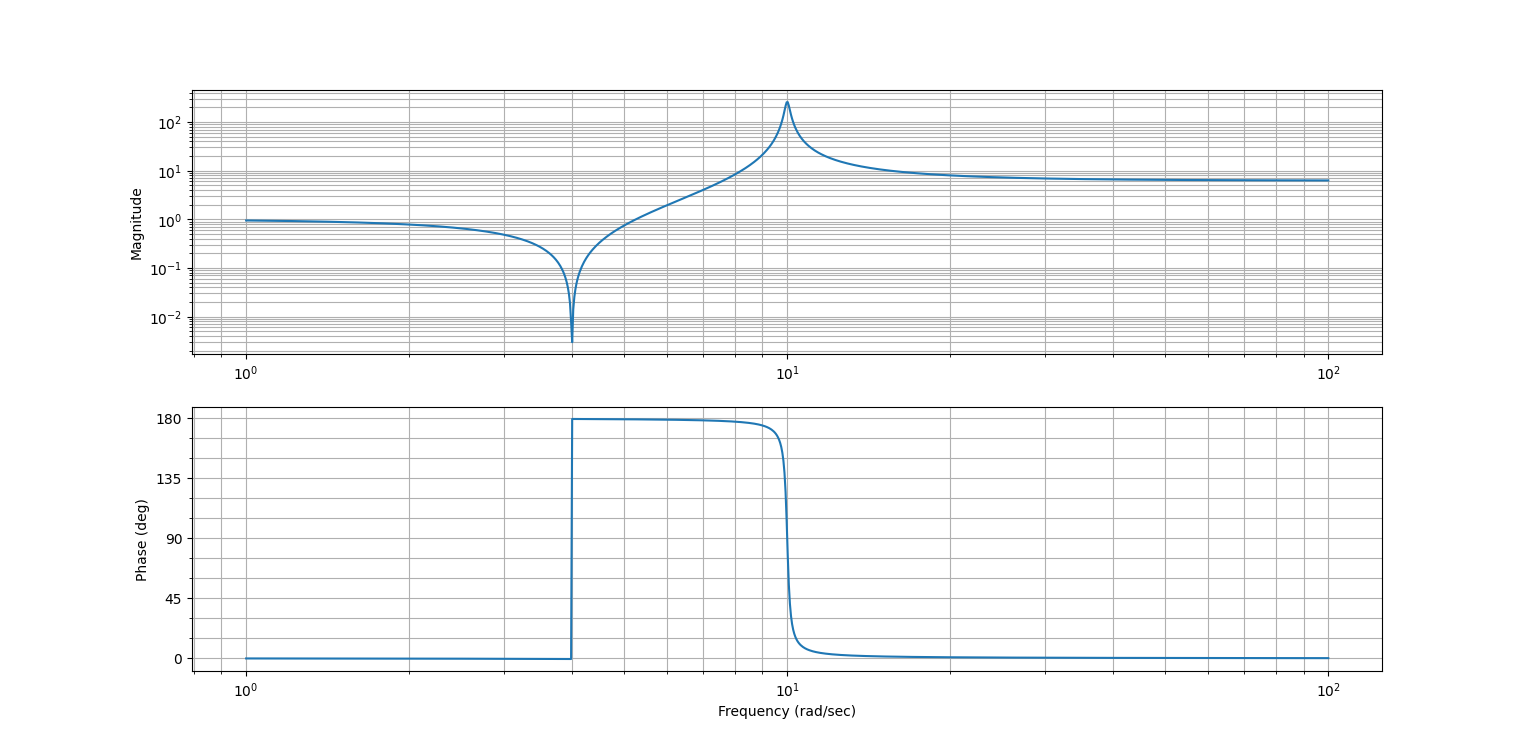
\includegraphics[scale=0.4]{bode.png}
    \caption{Diagrama de Bode}
\end{figure}

\begin{lstlisting}
import control as ctrl
import matplotlib.pyplot as plt
# 1. Definir a funcao de transferencia do sistema
num = [100, 0, 1600]  # numerador da funcao de transferencia
den = [16, 3.2, 1600]  # denominador da funcao de transferencia
H = ctrl.TransferFunction(num, den)
# 2. Plotar o diagrama de Bode
ctrl.bode_plot(H)
plt.show()    
\end{lstlisting}

\quad O diagrama de Bode é uma ferramenta muito útil,
usado para analisar o comportamento de um sistema em frequências diferentes.
Ele é usado para plotar a resposta em frequência de um sistema,
mostrando como a amplitude e a fase de um sinal de entrada mudam em relação à frequência.
Então, é possível observar pelo diagrama de Bode que haverá comportamento bem característicos nas frequências de 1 rad/s,
4 rad/s, 10 rad/s e 100 rad/s em suas magnitudes e fases,
que são justamente as frequências dos cossenos escolhidos para entrada do sistema nas questões propostas.

\quad Plotando o gráfico da resposta ao impulso $u(t) = \delta(t)$ em Python com o seguinte código:

\begin{figure}[h]
    \centering
    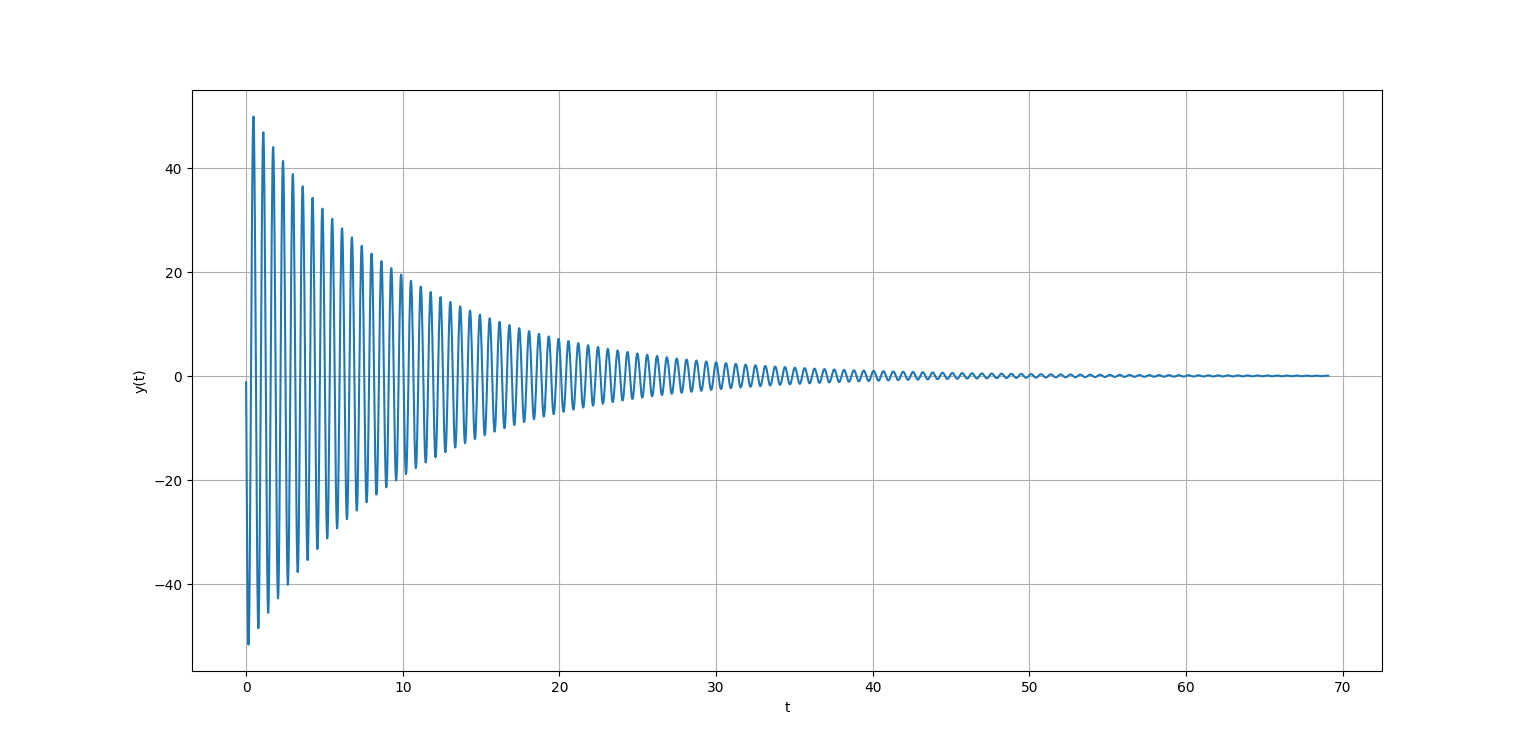
\includegraphics[scale=0.4]{impulso.png}
    \caption{Resposta ao impulso}
\end{figure}

\begin{lstlisting}
import numpy as np
import matplotlib.pyplot as plt
import control as ctrl
# 1. Definir a funcao de transferencia do sistema
num = [100, 0, 1600]  # numerador da funcao de transferencia
den = [16, 3.2, 1600]  # denominador da funcao de transferencia
sys = ctrl.TransferFunction(num, den)  # criar o objeto que representa o sistema
# 2. Calcular a resposta ao impulso
t, h = ctrl.impulse_response(sys)
# 3. Plotar do grafico da resposta ao impulso
plt.plot(t, h)
plt.xlabel('t(s)')
plt.ylabel('y(t)')
plt.grid()
plt.show()
\end{lstlisting}

\quad Observar o gráfico de resposta ao impulso de um sistema é importante porque ele fornece informações sobre como o sistema responde a um impulso de entrada.
No exemplo do trabalho, é possível perceber que a resposta ao impulso, é uma senoíde exponencialmente amortecida.

\quad Por meio da tabela, foi calculado o Laplace do cosseno de frequência $\omega$ multiplicado pelo degrau unitário:

\begin{equation}
    U(s) = \mathcal{L}\{ \cos(\omega t) 1(t) \} = \frac{s}{s^2 + \omega^2}
\end{equation}

\quad Calculando o Laplace da saída do sistema sem substituir o $\omega$ da fórmula acima:

\begin{equation}
    Y(s) = H(s)U(s) = \frac{100}{16} \frac{s^2 + 16}{s^2 + 0.2s + 100} \frac{s}{s^2 + \omega^2} = \frac{100}{16} \left[ \frac{k_1s + k_2}{s^2 + 0.2s + 100} + \frac{k_3s + k_4}{s^2 + \omega^2} \right] 
\end{equation}

\quad Para determinar os valores de $k_1$, $k_2$, $k_3$ e $k_4$, podemos igualar o numerador da função original aos numeradores das frações parciais:

\begin{equation}
    s^3 + 16s = k_1s^3 + k_2s^2 + k_1\omega^2 s + k_2\omega^2 + k_3s^3 + 0.2k_3s^2 + 100k_3s + k_4s^2 + 0.2k_4s + 100k_4
\end{equation}

\quad Montando o sistema de equações resultante com a frequência $\omega$ para ser substituído no desenvolvimento:

\begin{equation}
    \left\{
    \begin{array}{l}
        k_1 + k_3 = 1 \\
        k_2 + 0.2k_3 +k_4 = 0 \\
        \omega^2k_1 + 100k_3 + 0.2k_4 = 16 \\
        \omega^2k_2 + 100k_4 = 0
    \end{array}
    \right. 
\end{equation}

\newpage

\section{Desenvolvimento}

\quad 1. Foi considerado uma entrada $u(t) = cos(t) 1(t)$. Foi obtido a $y(t)$ por simulação numérica. Solução analítica ($\omega = 1$):

\begin{equation}
    \left\{
    \begin{array}{l}
        k_1 + k_3 = 1 \\
        k_2 + 0.2k_3 +k_4 = 0 \\
        k_1 + 100k_3 + 0.2k_4 = 16 \\
        k_2 + 100k_4 = 0
    \end{array}
    \right. 
\end{equation}

\quad Obtendo a solução do sistema, por meio da utilização da calculadora científica:

\begin{equation}
    k_1 = 0.8484; k_2 = -0.0306; k_3 = 0.1515; k_4 = 0.0003.
\end{equation}

\quad Substituindo $k_1$, $k_2$, $k_3$ e $k_4$ na Transformada de Laplace da saída $Y(s)$:

\begin{equation}
    Y(s) = \frac{100}{16} \left[ \frac{0.8484s -0.0306}{(s + 0.1)^2 + 99.99} + \frac{0.1515s + 0.0003}{s^2 + 1^2} \right]
\end{equation}

\quad Organizando a função para faciltar a aplicação da Transformada Inversa de Laplace:

\begin{equation}
    Y(s) = \frac{100}{16} \left[ \frac{0.8484(s + 0.1)}{(s + 0.1)^2 + 9.999^2} - \frac{0.0115 \cdot 9.999}{(s + 0.1)^2 + 9.999^2} +\frac{0.1515s}{s^2 + 1^2} + \frac{0.0003}{s^2 + 1^2} \right]
\end{equation}

\quad Aplicação da Transformada de Laplace Inversa para encontrar a saída $y(t)$:

\begin{equation}
    y(t) = \mathcal{L}^{-1} \{Y(s) \} = \frac{100}{16} \left[ 0.8484e^{-0.1t}cos(9.999t) - 0.0115e^{-0.1t}sin(9.999t) + 0.1515cos(t) + 0.0003sin(t) \right] 1(t)
\end{equation}

\begin{figure}[h]
    \centering
    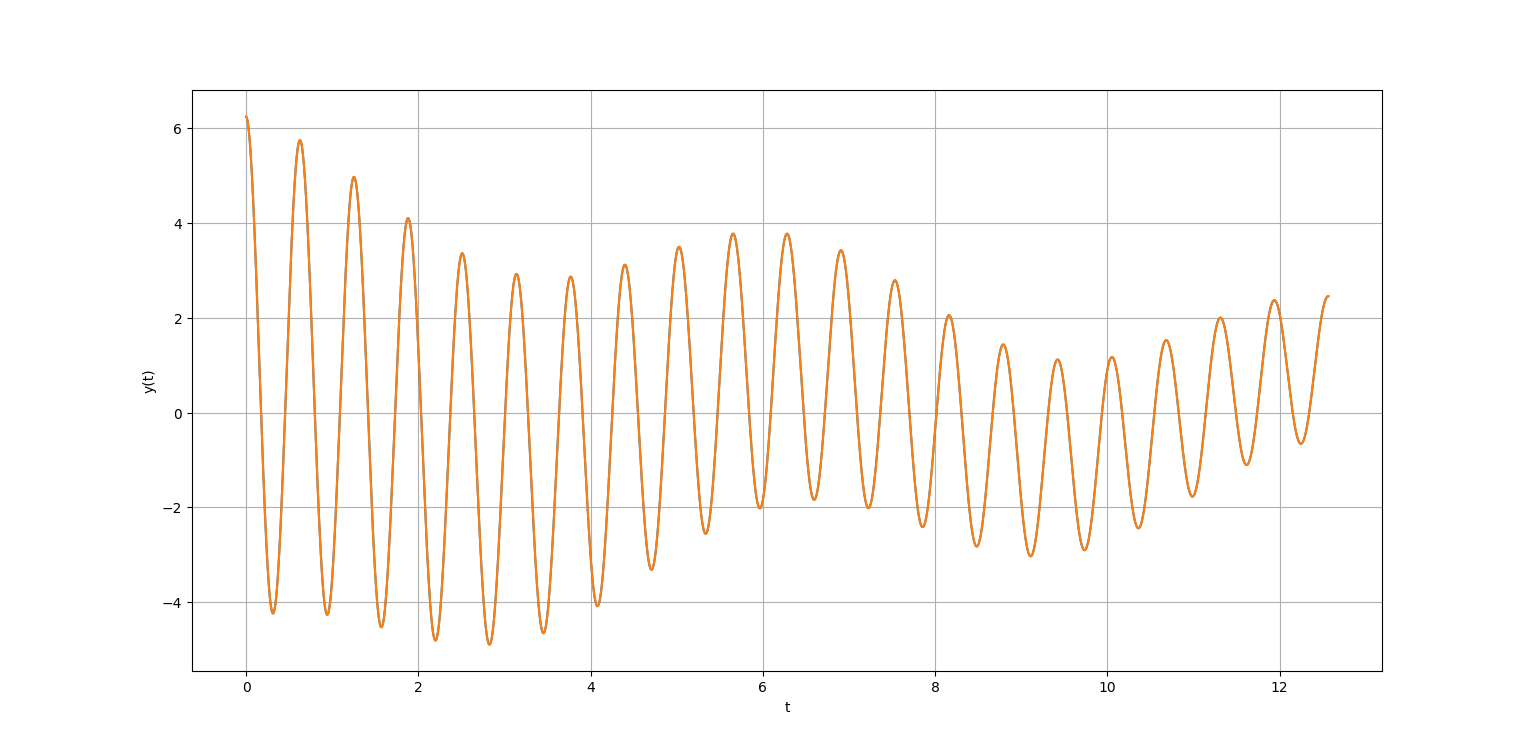
\includegraphics[scale=0.4]{questao1.png}
    \caption{Resposta ao cosseno com frequência 1 rad/s multiplicado pelo degrau unitario}
\end{figure}

\begin{lstlisting}
import numpy as np
import control as ctrl
import matplotlib.pyplot as plt
# 1. Definir a funcao de transferencia do sistema
num = [100, 0, 1600]  # numerador da funcao de transferencia
den = [16, 3.2, 1600]  # denominador da funcao de transferencia
sys = ctrl.TransferFunction(num, den)  # criar o objeto que representa o sistema
# 2. Definir os valores de tempo para simulacao
t = np.linspace(0, 4*np.pi, 10000)  # valores de tempo de 0 a 4*pi segundos
# 3. Definir o sinal de entrada como o cosseno multiplicado pelo degrau unitario
u = np.heaviside(t, 1) * np.cos(t)
# 4. Realizar a simulacao da resposta do sistema usando a funcao `control.forced_response()`
t_out, yout= ctrl.forced_response(sys, T=t, U=u)
# 5. Resposta analitica
y_a = 100/16*(0.8484*np.exp(-0.1*t)*np.cos(9.999*t)-0.0115*np.exp(-0.1*t)*np.sin(9.999*t) +
    0.1515*np.cos(t) + 0.0003*np.sin(t))
# 6. Plotar o grafico da resposta
plt.plot(t_out, yout)
plt.plot(t, y_a)
plt.xlabel('t')
plt.ylabel('y(t)')
plt.grid()
plt.show()
\end{lstlisting}

(a) A resposta coincide com o esperado na solução analítica?

\quad Sim, porque os valores obtidos graficamente da simulação numérica coincidiu bastante com a solução analítica.
Podendo observar essa coincidência entre os métodos pela Figura 3 em que os dois traçados dos gráficos se sobrepõem.
Além disso, é possível observar o comportamento tanto de senoídes quanto de senoídes exponencialmente amortecidas.

\quad Observando a Figura 4 a seguir, é possível observar que existe um erro quadrático considerável
ao percorrer um intervalo de 0 a 4$\pi$ que é causado tanto pela aproximação numérica feita pela linguagem Python e biblioteca Numpy
quanto pelo erro de arredondamento na solução analítica ao diminuir o número de algarismos significativos.

\begin{lstlisting}
    # 7. Calculando o erro quadratico
    y_error = (yout-y_a)**2
\end{lstlisting}

\newpage

\begin{figure}[h]
    \centering
    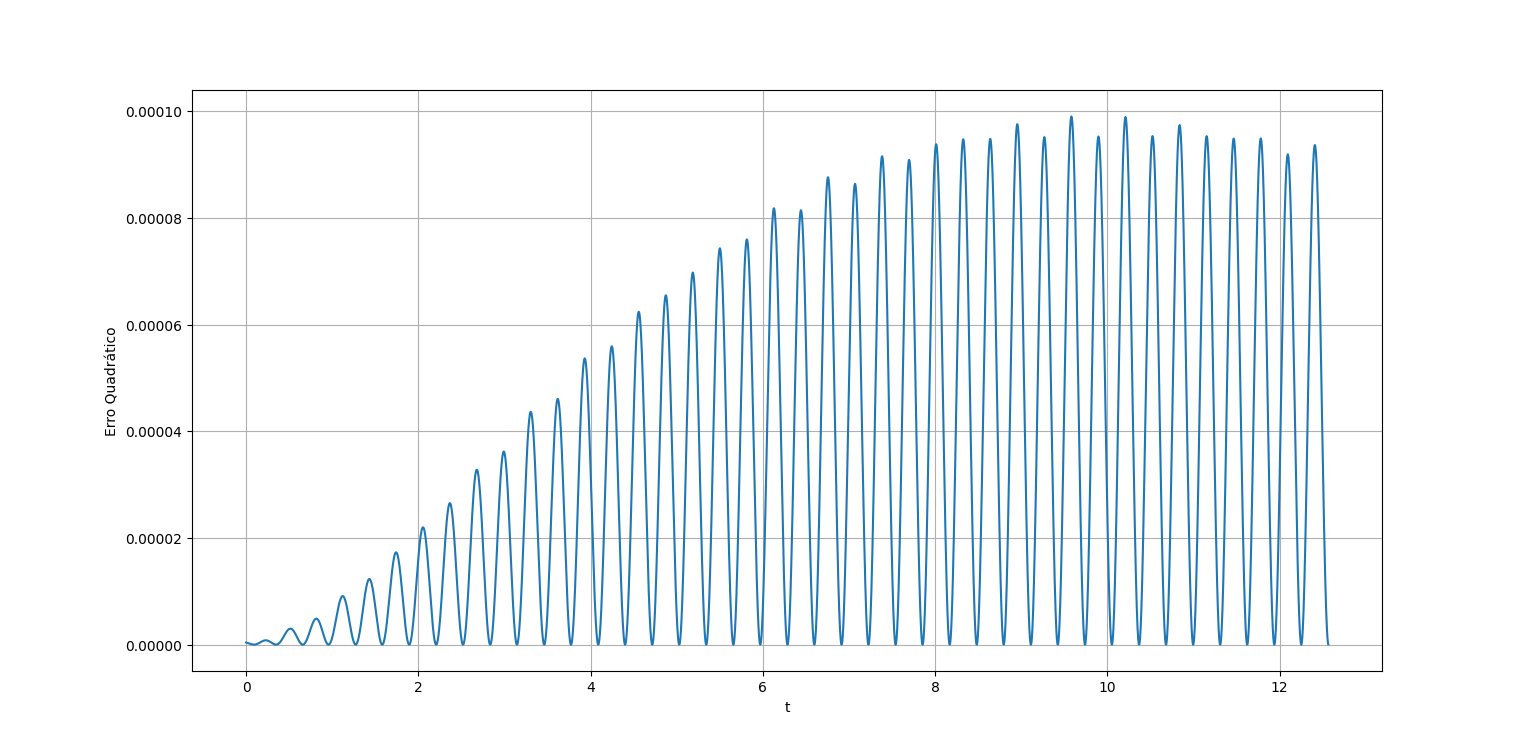
\includegraphics[scale=0.4]{erro1.png}
    \caption{Erro quadrático $(\omega = 1)$}
\end{figure}

(b) Que frequências aparecem na resposta? A que estâo associadas estas frequências?

\quad Observando a Figura 3, as frequências que aparecem na resposta são aproximadamente 1 rad/s e 9.999 rad/s.
A frequência 1 rad/s está relacionada a entrada $u(t) = $ que é um cosseno de frequência 1 rad/s.
Além disso, a frequência 9.999 rad/s está relacionada a função de transferência do sistema $H(s)$
que possui uma resposta ao impulso $\delta(t)$ sendo uma senoíde exponencialmente amortecida de frequência 9.999 rad/s.

\newpage

\quad 2. Foi considerado uma entrada $u(t) = cos(4 t) 1(t)$ (frequência de zero). Foi obtido a resposta $y(t)$ por simulação numérica. Solução analítica ($\omega = 4$):

\begin{equation}
    \left\{
    \begin{array}{l}
        k_1 + k_3 = 1 \\
        k_2 + 0.2k_3 +k_4 = 0 \\
        16k_1 + 100k_3 + 0.2k_4 = 16 \\
        16k_2 + 100k_4 = 0
    \end{array}
    \right. 
\end{equation}

\quad Obtendo a solução do sistema, por meio da utilização da calculadora científica:

\begin{equation}
    k_1 = 1; k_2 = 0; k_3 = 0; k_4 = 0.
\end{equation}

\quad Substituindo $k_1$, $k_2$, $k_3$ e $k_4$ na Transformada de Laplace da saída $Y(s)$.
Organizando a função para faciltar a aplicação da Transformada Inversa de Laplace:

\begin{equation}
    Y(s) = \frac{100}{16} \left[ \frac{s}{(s + 0.1)^2 + 99.99} \right] = \frac{100}{16} \left[ \frac{(s + 0.1)}{(s + 0.1)^2 + 9.999^2} - \frac{0.01 \cdot 9.999}{(s + 0.1)^2 + 9.999^2} \right]
\end{equation}

\quad Aplicação da Transformada de Laplace Inversa para encontrar a saída $y(t)$:

\begin{equation}
    y(t) = \mathcal{L}^{-1} \{Y(s) \} = \frac{100}{16} \left[ e^{-0.1t}cos(9.999t) - 0.01e^{-0.1t}sin(9.999t) \right] 1(t)
\end{equation}

\begin{figure}[h]
    \centering
    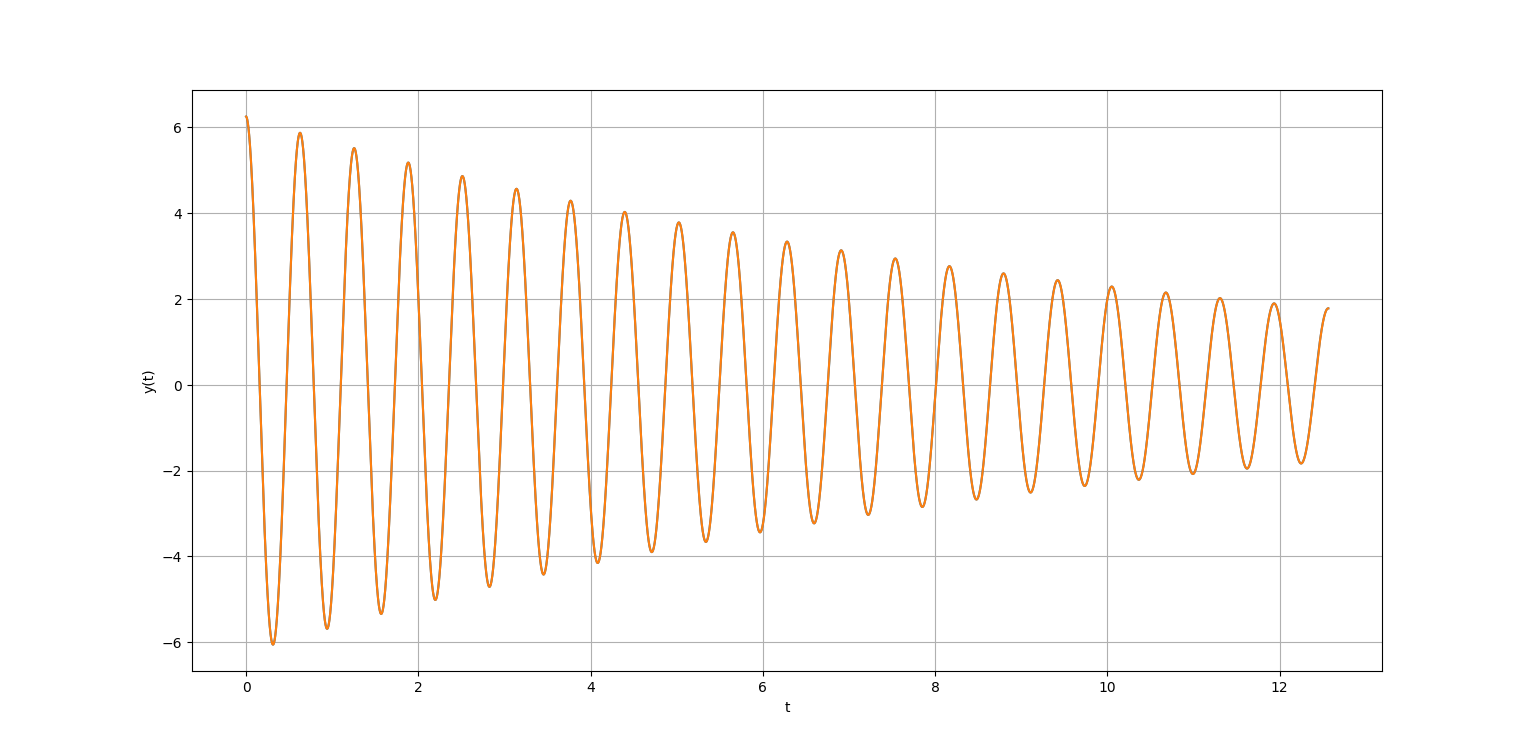
\includegraphics[scale=0.4]{questao2.png}
    \caption{Resposta ao cosseno com frequência 4 rad/s multiplicado pelo degrau unitario}
\end{figure}


\begin{lstlisting}
import numpy as np
import control as ctrl
import matplotlib.pyplot as plt
# 1. Definir a funcao de transferencia do sistema
num = [100, 0, 1600]  # numerador da funcao de transferencia
den = [16, 3.2, 1600]  # denominador da funcao de transferencia
sys = ctrl.TransferFunction(num, den)  # criar o objeto que representa o sistema
# 2. Definir os valores de tempo para simulacao
t = np.linspace(0, 4*np.pi, 10000)  # valores de tempo de 0 a 4*pi segundos
# 3. Definir o sinal de entrada como o cosseno multiplicado pelo degrau unitario
u = np.heaviside(t, 1) * np.cos(4*t)
# 4. Realizar a simulacao da resposta do sistema usando a funcao `control.forced_response()`
t_out, yout= ctrl.forced_response(sys, T=t, U=u)
# 5. Resposta analitica
y_a = 100/16*(np.exp(-0.1*t)*np.cos(9.999*t)-0.01*np.exp(-0.1*t)*np.sin(9.999*t))
# 6. Plotar o grafico da resposta
plt.plot(t_out, yout)
plt.plot(t, y_a)
plt.xlabel('t')
plt.ylabel('y(t)')
plt.show()
\end{lstlisting}

(a) A resposta coincide com o esperado na solução analítica?

\quad Sim, porque os valores obtidos graficamente da simulação numérica coincidiu bastante com a solução analítica.
Podendo observar essa coincidência entre os métodos pela Figura 5 em que os dois traçados dos gráficos se sobrepõem.
Além disso, é possível observar o comportamento de uma senoíde exponencialmente amortecida.

\quad Observando a Figura 6 a seguir, é possível observar que existe um erro quadrático considerável
ao percorrer um intervalo de 0 a 4$\pi$ que é causado tanto pela aproximação numérica feita pela linguagem Python e biblioteca Numpy
quanto pelo erro de arredondamento na solução analítica ao diminuir o número de algarismos significativos.

\begin{lstlisting}
    # 7. Calculando o erro quadratico
    y_error = (yout-y_a)**2
\end{lstlisting}

\newpage

\begin{figure}[h]
    \centering
    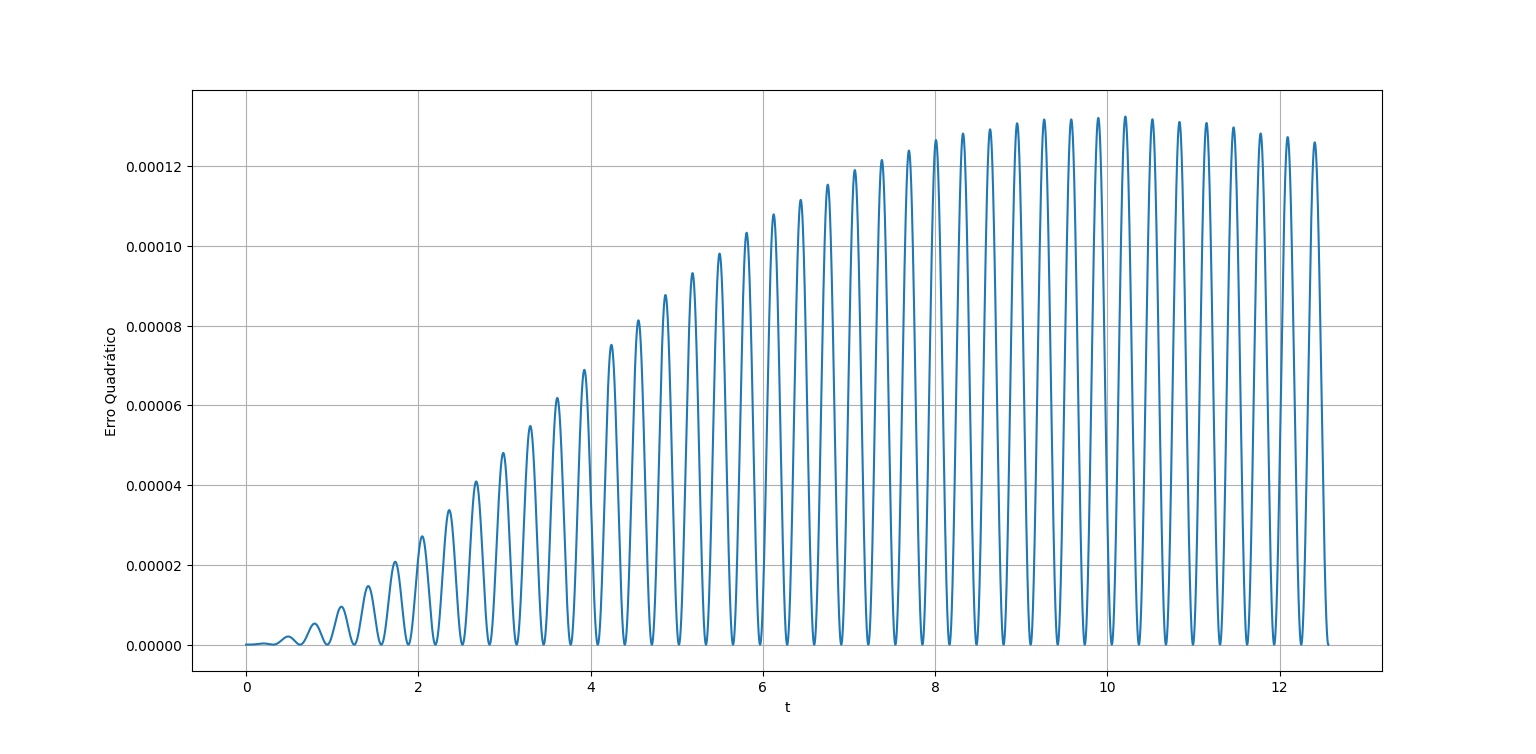
\includegraphics[scale=0.4]{erro2.png}
    \caption{Erro quadrático $(\omega = 4)$}
\end{figure}

(b) Que frequências aparecem na resposta? A que estâo associadas estas frequências?

\quad Observando a Figura 5, a única frequência que aparece na resposta é aproximadamente 9.999 rad/s.
A frequência 9.999 rad/s está relacionada a função de transferência do sistema
que possui uma resposta ao impulso $\delta(t)$ sendo uma senoíde exponencialmente amortecida.

(c) Aparece a frequência 4 rad/s na resposta? Caso negativo, porque?

\quad Não aparece a frequência 4 rad/s na resposta. Porque, os zeros da função de transferência afetam a resposta em frequência do sistema,
anulando a amplitude da resposta nessa frequência específica.
Quando a entrada é um cosseno com frequência igual a 4 rad/s,
a função de transferência do sistema irá multiplicar essa entrada pelos fatores (s - 4j) e (s + 4j).
Como ambos os zeros estão localizados em $\pm$ 4j na parte imaginária do plano complexo,
esses fatores serão iguais a zero na frequência de 4 rad/s,
o que significa que a resposta do sistema a essa frequência será nula.

\newpage

\quad 3. Foi considerado uma entrada $u(t) = cos(10 t) 1(t)$. Foi obtido a resposta $y(t)$ por simulação numérica. Solução analítica ($\omega = 10$):

\begin{equation}
    \left\{
    \begin{array}{l}
        k_1 + k_3 = 1 \\
        k_2 + 0.2k_3 +k_4 = 0 \\
        100k_1 + 100k_3 + 0.2k_4 = 16 \\
        100k_2 + 100k_4 = 0
    \end{array}
    \right. 
\end{equation}

\quad Obtendo a solução do sistema, por meio da utilização da calculadora científica:

\begin{equation}
    k_1 = 1; k_2 = 420; k_3 = 0; k_4 = -420.
\end{equation}

\quad Substituindo $k_1$, $k_2$, $k_3$ e $k_4$ na Transformada de Laplace da saída $Y(s)$:

\begin{equation}
    Y(s) = \frac{100}{16} \left[ \frac{s+420}{(s + 0.1)^2 + 99.99} - \frac{420}{s^2 + 10^2} \right]
\end{equation}

\quad Organizando a função para faciltar a aplicação da Transformada Inversa de Laplace:

\begin{equation}
    Y(s) = \frac{100}{16} \left[ \frac{(s + 0.1)}{(s + 0.1)^2 + 9.999^2} + \frac{41.9941 \cdot 9.999}{(s + 0.1)^2 + 9.999^2} - \frac{42 \cdot 10}{s^2 + 10^2} \right]
\end{equation}

\quad Aplicação da Transformada de Laplace Inversa para encontrar a saída $y(t)$:

\begin{equation}
    y(t) = \mathcal{L}^{-1} \{Y(s) \} = \frac{100}{16} \left[ e^{-0.1t}cos(9.999t) + 41.9941e^{-0.1t}sin(9.999t) - 42sin(10t) \right] 1(t)
\end{equation}

\begin{figure}[h]
    \centering
    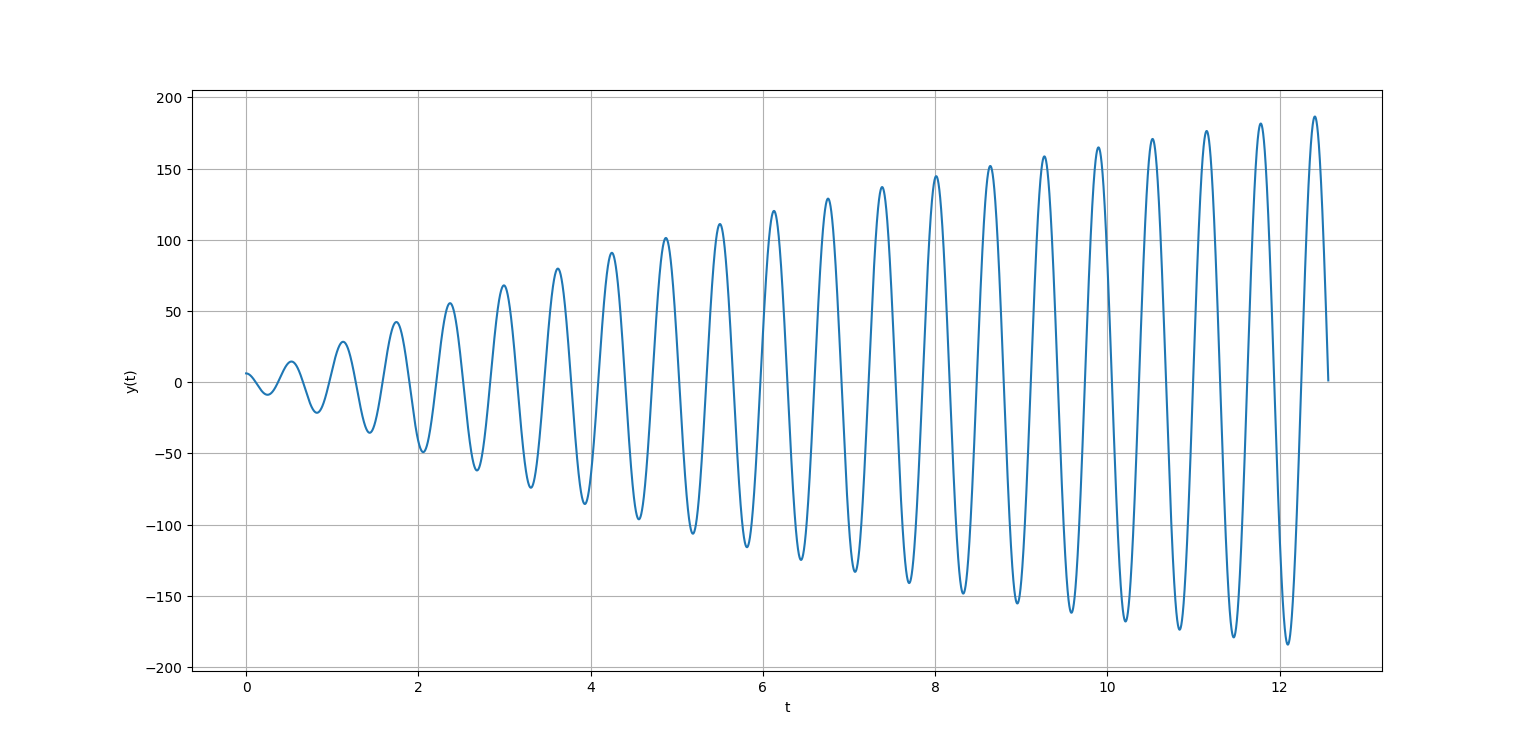
\includegraphics[scale=0.4]{questao3.png}
    \caption{Resposta ao cosseno com frequência 10 rad/s multiplicado pelo degrau unitario}
\end{figure}

\begin{lstlisting}
import numpy as np
import control as ctrl
import matplotlib.pyplot as plt
# 1. Definir a funcao de transferencia do sistema
num = [100, 0, 1600]  # numerador da funcao de transferencia
den = [16, 3.2, 1600]  # denominador da funcao de transferencia
sys = ctrl.TransferFunction(num, den)  # criar o objeto que representa o sistema
# 2. Definir os valores de tempo para simulacao
t = np.linspace(0, 4*np.pi, 10000)  # valores de tempo de 0 a 4*pi segundos
# 3. Definir o sinal de entrada como o cosseno multiplicado pelo degrau unitario
u = np.heaviside(t, 1) * np.cos(10*t)
# 4. Realizar a simulacao da resposta do sistema usando a funcao `control.forced_response()`
t_out, yout= ctrl.forced_response(sys, T=t, U=u)
# 5. Resposta analitica
y_a = 100/16*(np.exp(-0.1*t)*np.cos(9.999*t)+41.9941*np.exp(-0.1*t)*np.sin(9.999*t)-
    42*np.sin(10*t))
# 6. Plotar o grafico da resposta
plt.plot(t_out, yout)
plt.plot(t, y_a)
plt.xlabel('t')
plt.ylabel('y(t)')
plt.show()
\end{lstlisting}

(a) A resposta coincide com o esperado na solução analítica?

\quad Sim, porque os valores obtidos graficamente da simulação numérica coincidiu bastante com a solução analítica.
Podendo observar essa coincidência entre os métodos pela Figura 7 em que os dois traçados dos gráficos se sobrepõem.

\quad Observando a Figura 8 a seguir, é possível observar que existe um erro quadrático 10 vezes maior que os demais
ao percorrer um intervalo de 0 a 4$\pi$ que é causado tanto pela aproximação numérica feita pela linguagem Python e biblioteca Numpy
quanto pelo erro de arredondamento na solução analítica ao diminuir o número de algarismos significativos.

\begin{lstlisting}
    # 7. Calculando o erro quadratico
    y_error = (yout-y_a)**2
\end{lstlisting}

\newpage

\begin{figure}[h]
    \centering
    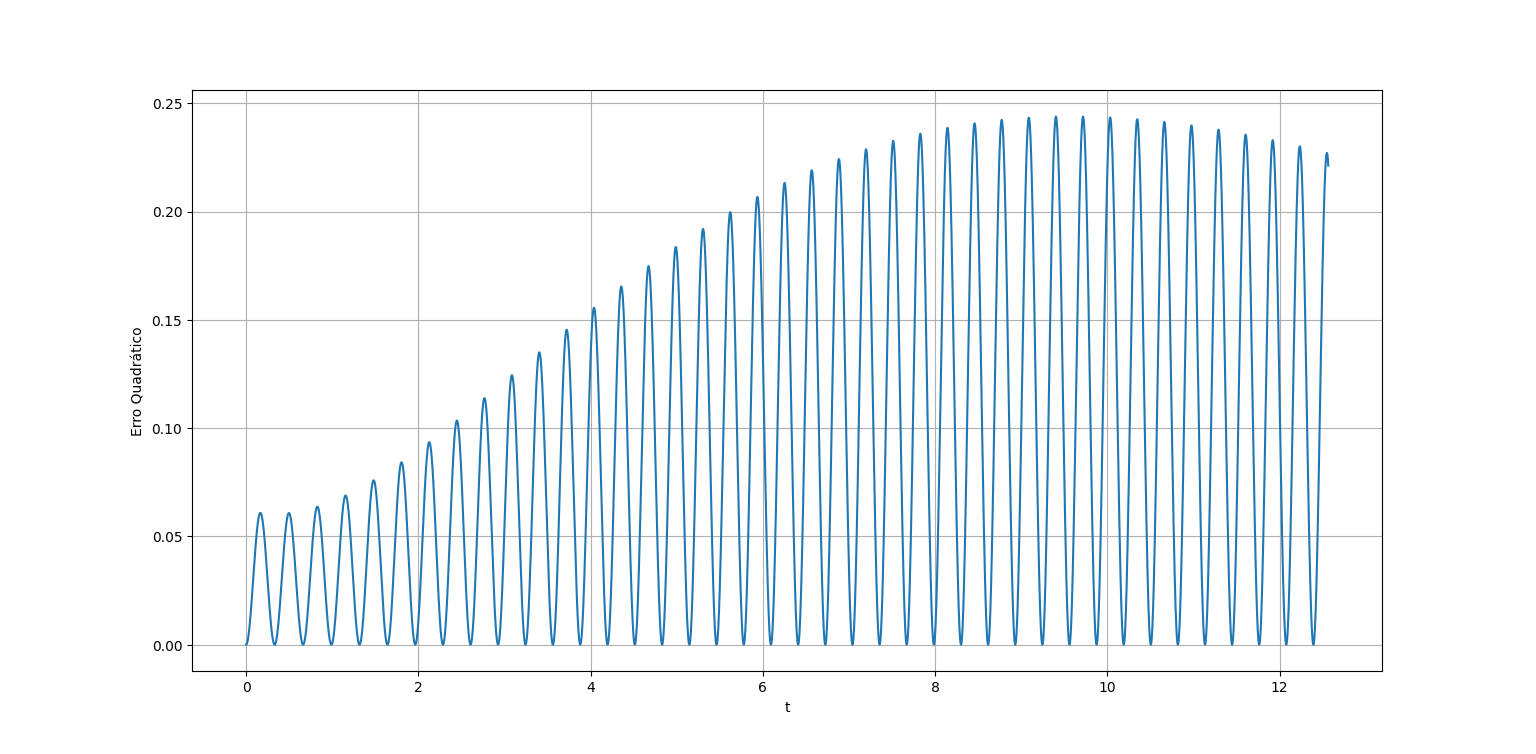
\includegraphics[scale=0.4]{erro3.png}
    \caption{Erro quadrático $(\omega = 10)$}
\end{figure}

(b) Que frequências aparecem na resposta? A que estâo associadas estas frequências?

\quad As frequências que aparecem na resposta são aproximadamente 10 rad/s e 9.999 rad/s.
A frequência 10 rad/s está relacionada a entrada $u(t) = cos(10t) 1(t)$ que é um cosseno de frequência 10 rad/s.
Além disso, a frequência 9.999 rad/s está relacionada a função de transferência do sistema $H(s)$
que possui uma resposta ao impulso $\delta(t)$ sendo uma senoíde exponencialmente amortecida.
Porém, é muito difícil distinguir as duas freqûencias pelo fato de terem valores muito próximos e
estarem em fase. Mesmo que seja aumentado o intervalo de amostragem ainda seria muito difícil de visualizar.

\newpage

\quad 4. Foi considerado uma entrada $u(t) = cos(100 t) 1(t)$. Foi obtido a resposta $y(t)$ por simulação numérica. Solução analítica ($\omega = 100$):

\begin{equation}
    \left\{
    \begin{array}{l}
        k_1 + k_3 = 1 \\
        k_2 + 0.2k_3 +k_4 = 0 \\
        10000k_1 + 100k_3 + 0.2k_4 = 16 \\
        10000k_2 + 100k_4 = 0
    \end{array}
    \right. 
\end{equation}

\quad Obtendo a solução do sistema, por meio da utilização da calculadora científica:

\begin{equation}
    k_1 = -0.0085; k_2 = 0.0020; k_3 = 1.0085; k_4 = -0.2037.
\end{equation}

\quad Substituindo $k_1$, $k_2$, $k_3$ e $k_4$ na Transformada de Laplace da saída $Y(s)$:

\begin{equation}
    Y(s) = \frac{100}{16} \left[ \frac{-0.0085s+0.0020}{(s + 0.1)^2 + 99.99} + \frac{1.0085s -0.2037}{s^2 + 100^2} \right]
\end{equation}

\quad Organizando a função para faciltar a aplicação da Transformada Inversa de Laplace:

\begin{equation}
    Y(s) = \frac{100}{16} \left[-\frac{0.0085(s + 0.1)}{(s + 0.1)^2 + 9.999^2} + \frac{0.0010 \cdot 9.999}{(s + 0.1)^2 + 9.999^2} + \frac{1.0085s}{s^2 + 100^2} - \frac{0.0002 \cdot 100}{s^2 + 100^2} \right]
\end{equation}

\quad Aplicação da Transformada de Laplace Inversa para encontrar a saída $y(t)$:

\begin{equation}
    y(t) = \mathcal{L}^{-1} \{Y(s) \} = \frac{100}{16} \left[-0.0085e^{-0.1t}cos(9.999t)+0.0010e^{-0.1t}sin(9.999t) + 1.0085cos(100t) - 0.0002sin(100t) \right] 1(t)
\end{equation}

\begin{figure}[h]
    \centering
    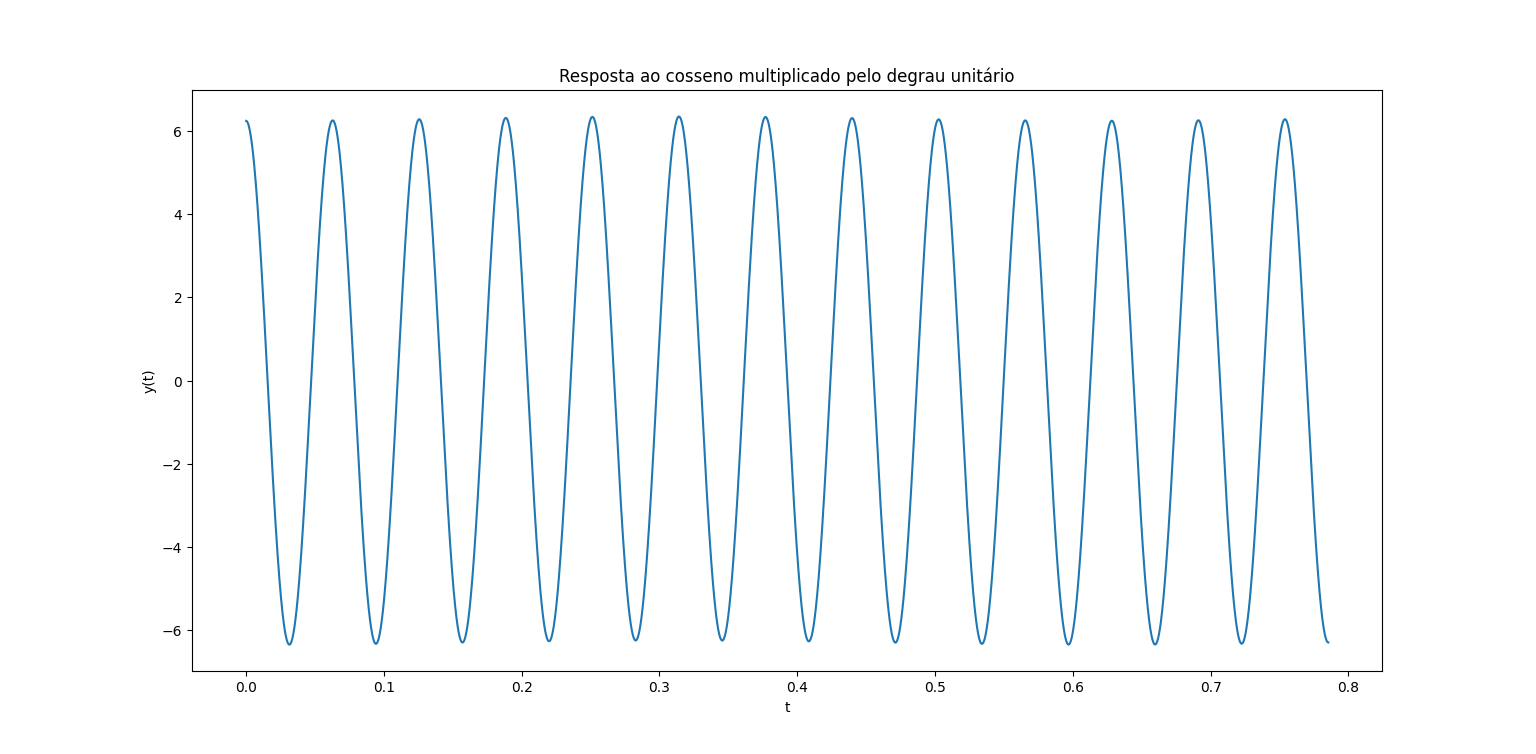
\includegraphics[scale=0.4]{questao4.png}
    \caption{Resposta ao cosseno com frequência 100 rad/s multiplicado pelo degrau unitario}
\end{figure}

\begin{figure}[h]
    \centering
    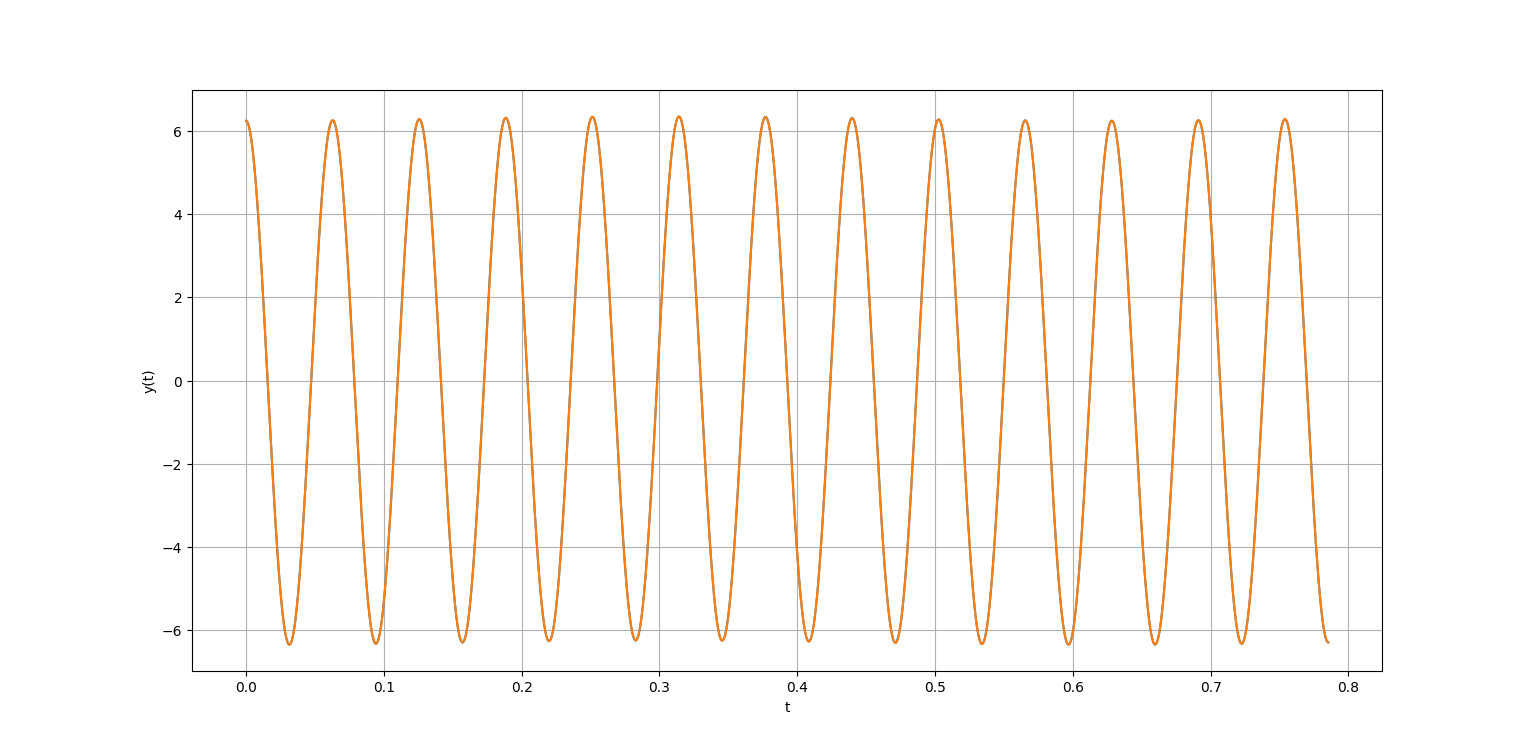
\includegraphics[scale=0.4]{questao4_zoom.png}
    \caption{Resposta com um intervalo de 0 a $\pi/4$}
\end{figure}

\begin{lstlisting}
import numpy as np
import control as ctrl
import matplotlib.pyplot as plt
# 1. Definir a funcao de transferencia do sistema
num = [100, 0, 1600]  # numerador da funcao de transferencia
den = [16, 3.2, 1600]  # denominador da funcao de transferencia
sys = ctrl.TransferFunction(num, den)  # criar o objeto que representa o sistema
# 2. Definir os valores de tempo para simulacao
t = np.linspace(0, 4*np.pi, 10000)  # valores de tempo de 0 a 4*pi segundos
# 3. Definir o sinal de entrada como o cosseno multiplicado pelo degrau unitario
u = np.heaviside(t, 1) * np.cos(100*t)
# 4. Realizar a simulacao da resposta do sistema usando a funcao `control.forced_response()`
t_out, yout = ctrl.forced_response(sys, T=t, U=u)
# 5. Resposta analitica
y_a = 100/16*(-0.0085*np.exp(-0.1*t)*np.cos(9.999*t)+0.0010*np.exp(-0.1*t)*np.sin(9.999*t)+
    1.0085*np.cos(100*t)-0.0002*np.sin(100*t))
# 6. Plotar o grafico da resposta
plt.plot(t_out, yout)
plt.plot(t, y_a)
plt.xlabel('t')
plt.ylabel('y(t)')
plt.show()
\end{lstlisting}

(a) A resposta coincide com o esperado na solução analítica?

\quad Sim, porque os valores obtidos graficamente da simulação numérica coincidiu bastante com a solução analítica.
Podendo observar essa coincidência entre os métodos pelas Figuras 9 e 10 em que os dois traçados dos gráficos se sobrepõem.
Além disso, é possível observar o comportamento tanto de senoídes quanto de senoídes exponencialmente amortecidas.

\quad Observando a Figura 11 a seguir, é possível observar que existe um erro quadrático considerável
ao percorrer um intervalo de 0 a 4$\pi$ que é causado tanto pela aproximação numérica feita pela linguagem Python e biblioteca Numpy
quanto pelo erro de arredondamento na solução analítica ao diminuir o número de algarismos significativos.
Porém, esse erro quadrático é inferior aos casos interiores.

\begin{lstlisting}
    # 7. Calculando o erro quadratico
    y_error = (yout-y_a)**2
\end{lstlisting}

\begin{figure}[h]
    \centering
    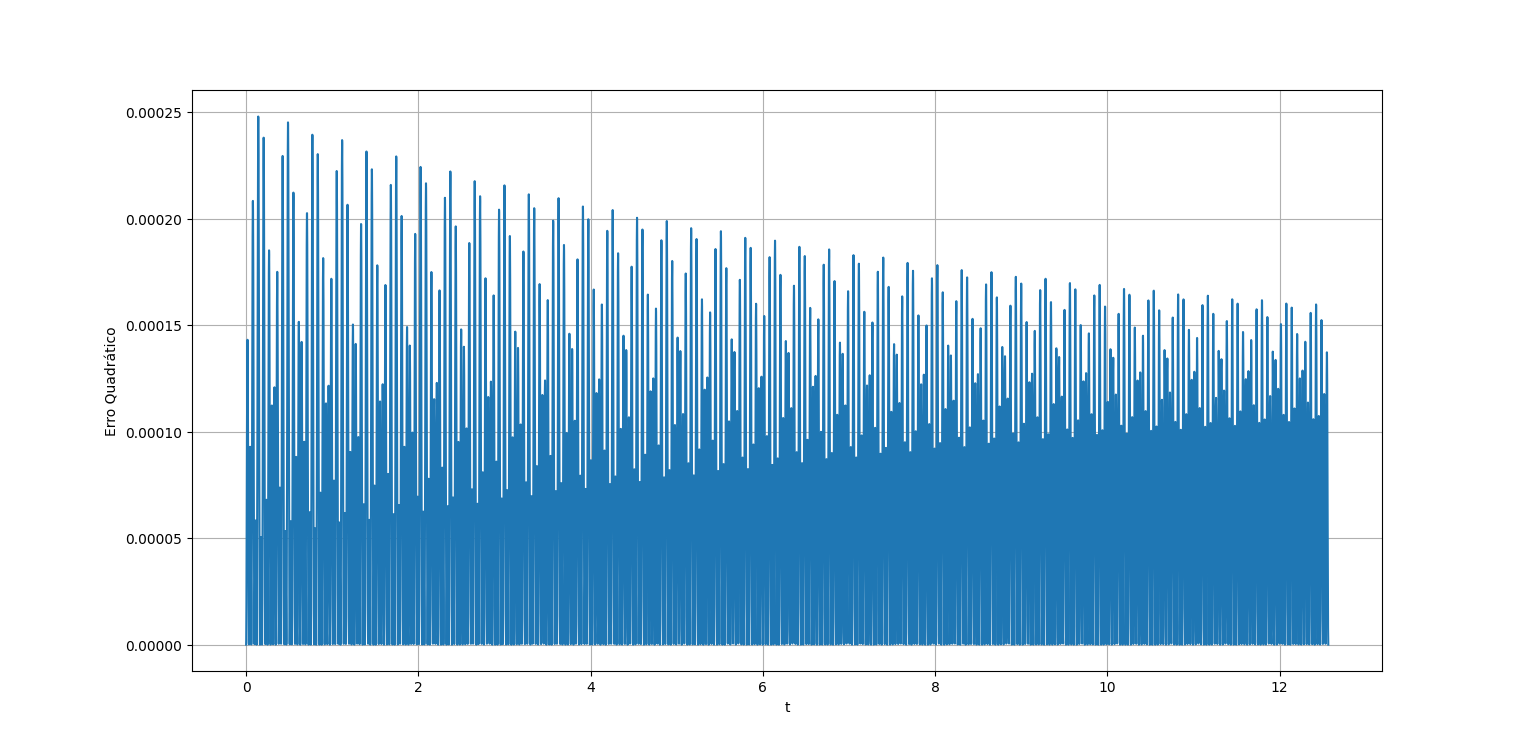
\includegraphics[scale=0.4]{erro4.png}
    \caption{Erro quadrático $(\omega = 100)$}
\end{figure}

(b) Que frequências aparecem na resposta? A que estâo associadas estas frequências?

\quad Observando as figuras 9 e 10, as frequências que aparecem na resposta são aproximadamente 100 rad/s e 9.999 rad/s.
A frequência 100 rad/s está relacionada a entrada $u(t) = cos(100t) 1(t)$ que é um cosseno de frequência 100 rad/s.
Além disso, a frequência 9.999 rad/s está relacionada a função de transferência do sistema $H(s)$
que possui uma resposta ao impulso $\delta(t)$ sendo uma senoíde exponencialmente amortecida.
Só foi possível observar essas duas frequências,
porque foram utilizados dois gráficos com intervalos diferentes de amostragem.


\newpage

\section{Conclusão}

\quad A conclusão é que os pólos e zeros de um sistema linear têm um impacto significativo em sua resposta.
A localização dos pólos determina a estabilidade do sistema e a rapidez com que ele responde a uma entrada.
Se os pólos estiverem na parte direita do plano complexo, o sistema é instável e não pode ser usado em aplicações práticas.
Por outro lado, se os pólos estiverem na parte esquerda do plano complexo, o sistema é estável e pode ser utilizado em aplicações práticas.
Esse é o caso sistema linear do trabalho que possui dois pólos complexos conjugados com parte real negativa ($p_1 = -0.1 + 9.9995j$ e $p_2 = -0.1 - 9.9995j$).

\quad Além disso, a localização dos pólos também afeta a rapidez com que o sistema responde a uma entrada.
Quanto mais longe os pólos estiverem do eixo imaginário, mais rápido será a resposta do sistema. Por outro lado,
os zeros afetam a forma como o sistema responde a diferentes frequências de entrada.
Um zero em uma frequência específica anula a resposta do sistema a essa frequência
(o que ocorre na questão 2.(c)),
enquanto um zero próximo a uma frequência específica pode reduzir a amplitude da resposta do sistema a essa frequência.

\quad Portanto, entender a localização dos pólos e zeros em um sistema linear é crucial para projetar sistemas estáveis e prever sua resposta a diferentes entradas.
\newpage

\section{Extras}

\quad Plotando o Diagrama de Nyquist em Python com o seguinte código (Feito por curiosidade):

\begin{figure}[h]
    \centering
    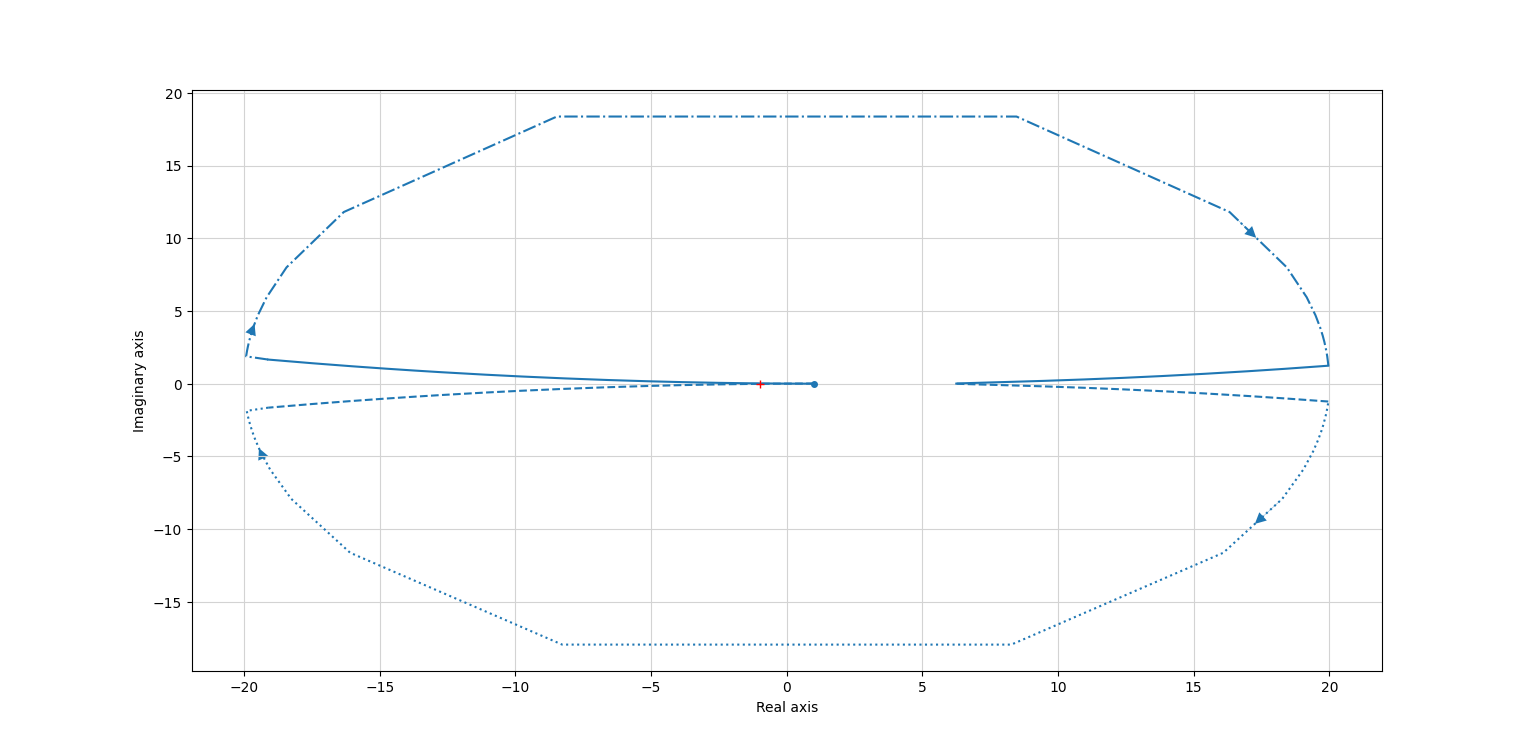
\includegraphics[scale=0.45]{nyquist.png}
    \caption{Diagrama de Nyquist}
\end{figure}

\begin{lstlisting}
import control as ctrl
import matplotlib.pyplot as plt
# 1. Definir a funcao de transferencia do sistema
num = [100, 0, 1600]  # numerador da funcao de transferencia
den = [16, 3.2, 1600]  # denominador da funcao de transferencia
H = ctrl.TransferFunction(num, den)
# 2. Plotar o diagrama de Nyquist
ctrl.nyquist_plot(H)
plt.show()
\end{lstlisting}

\newpage

\quad Plotando o Diagrama de Nichols em Python com o seguinte código (Feito por curiosidade):

\begin{figure}[h]
    \centering
    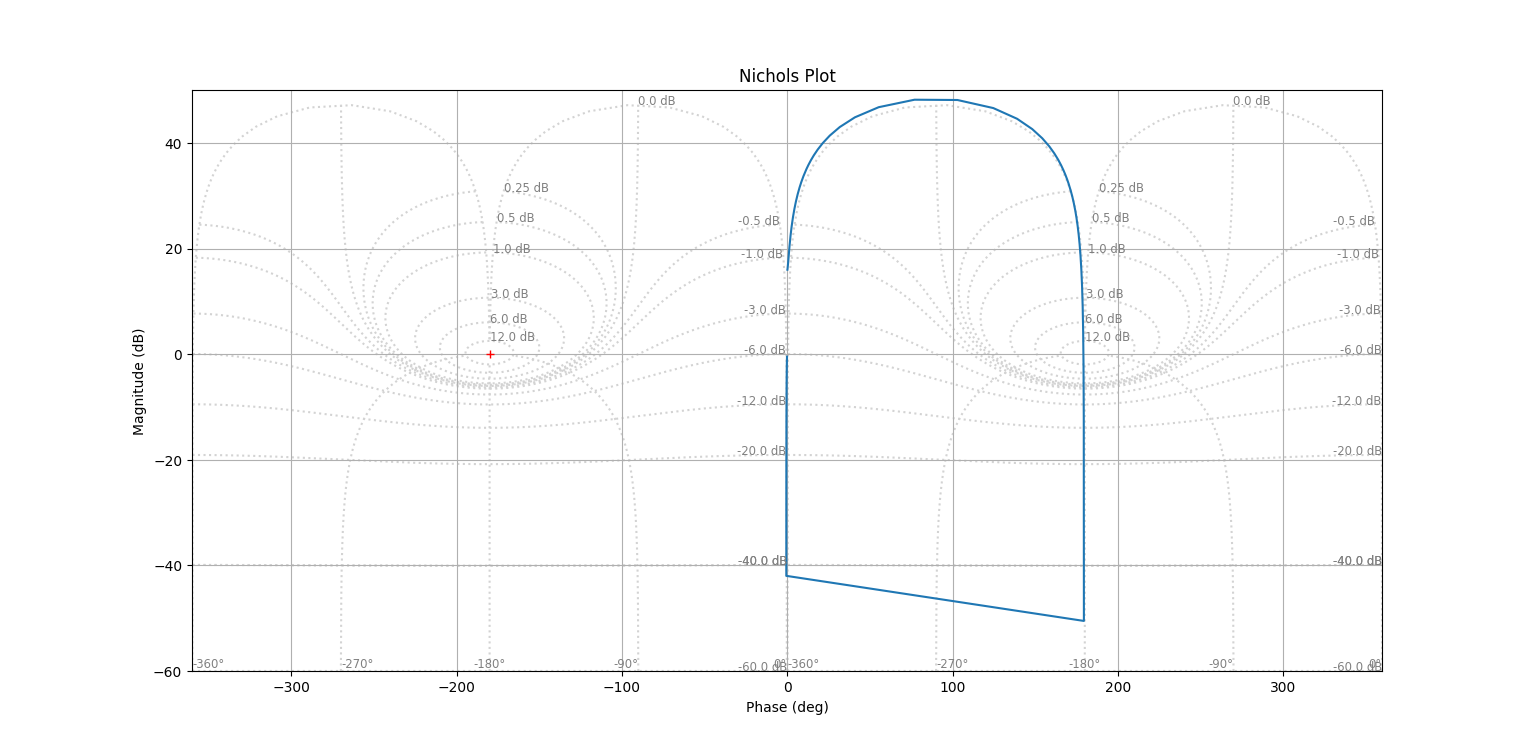
\includegraphics[scale=0.45]{nichols.png}
    \caption{Diagrama de Nichols}
\end{figure}

\begin{lstlisting}
import control as ctrl
import matplotlib.pyplot as plt
# 1. Definir a funcao de transferencia do sistema
num = [100, 0, 1600]  # numerador da funcao de transferencia
den = [16, 3.2, 1600]  # denominador da funcao de transferencia
H = ctrl.TransferFunction(num, den)
# 2. Plotar o diagrama de Nichols
ctrl.nichols_plot(H)
plt.grid()
plt.show()
\end{lstlisting}

\newpage

\begin{thebibliography}{99}
    \bibitem{pythoncontrol} Documentação do Python Control. Disponível em: \url{https://python-control.readthedocs.io/en/0.9.3.post2/}. Acesso em: 06 de maio de 2023.
    
    \bibitem{numpy} Documentação do NumPy. Disponível em: \url{https://numpy.org/doc/stable/}. Acesso em: 06 de maio de 2023.
    
    \bibitem{matplotlib} Documentação do Matplotlib. Disponível em: \url{https://matplotlib.org/stable/api/index}. Acesso em: 06 de maio de 2023.

    \bibitem{lathi} LATHI, B.P. \textit{Linear Systems and Signals}. 3rd ed. Oxford: Oxford University Press, 2018.

    \bibitem{delnero} GOMES, A.C.N. Notas de Aula - Sinais e Sistemas (COE350). Universidade Federal do Rio de Janeiro, Rio de Janeiro, RJ, Brasil, 2022. Disponível em: \url{http://coep.ufrj.br/~afel/notas.pdf}. Acesso em: 06 de maio de 2023.
\end{thebibliography}

\end{document}
